\chapter{机器学习的基础理论}\label{chap:ml_theory}

本章首先介绍了机器学习的基本概念(第\ref{sec:ml_intro}节);接着介绍论文中涉及的机器学习算法的基础理论,包括LR(第\ref{sec:ml_lr}节)、KNN(第\ref{sec:ml_knn}节)、DT(第\ref{sec:ml_dt}节)、RF(第\ref{sec:ml_rf}节)、ETR(第\ref{sec:ml_etr}节)、GBRT(第\ref{sec:ml_gbr}节)、SVR(第\ref{sec:ml_svr}节)、CNN(第\ref{sec:ml_cnn}节)、LSTM-RNN(第\ref{sec:ml_lstm}节);然后引出这些算法训练前的必要准备,包括滑动窗口法(第\ref{sec:ml_slide}节)、数据归一化(第\ref{sec:ml_scaler}节)、优化器(第\ref{sec:ml_optimizer}节)、优化目标函数(第\ref{sec:ml_loss}节)、性能度量(第\ref{sec:ml_performance}节)、欠拟合和过拟合(第\ref{sec:ml_fitting}节)、计算工具与平台(第\ref{sec:ml_computer}节)。

\section{引言}\label{sec:ml_intro}

本质上,各类算法设计的初衷是为解决某一特定任务。若想将某一种算法迁移到其他任务中,可能需要再次耗费大量的精力重新修缮算法。机器学习算法从大量样本中学习,若想将训练好的机器学习算法迁移到其他类似的任务上,只需要在原算法的基础上稍微进行调整训练。因此,即使面临的任务有所差异,学到的算法仍具有一定的通用性\citep{Goodfellow2016Deep}。

机器学习从数据中提取知识。或者说,机器学习是一种从数据中学习经验的算法。\citet{Mitchell1997Machine}将机器学习定义为:“假设性能$P$用来评估计算机计算的某类任务$T$,若该计算利用经验$E$在任务$T$上性能$P$有所提升,则对于$T$和$P$而言,计算机程序从$E$进行了有效的学习。”

传统的机器学习从训练样本出发,试图通过数据本身而不是原理分析获得规律,实现对数据行为或趋势的准确预测。机器学习通过平衡学习结果的有效性与学习算法的可解释性,为解决有限样本的学习任务提供了研究范式。本论文的研究方法将重点集中在监督学习算法上。被标记的数据可来自实际观测,也可来自数值模拟计算。基于这些被标记的数据集,使用监督学习算法挖掘数据中隐藏的信息,从而利用评估良好的算法预测未来趋势。

\section{机器学习算法}\label{sec:ml}

假设数据集为$D=\{(\Vector{x}_1,\Vector{y}_1),(\Vector{x}_2,\Vector{y}_2),\ldots,(\Vector{x}_m,\Vector{y}_m)\}$,其中$\Vector{X}=\{\Vector{x}_1,\Vector{x}_2,\ldots,\Vector{x}_m\}$,$\Vector{X}$为输入向量,$\Vector{x}_i\in\Vector{X}$为输入特征空间,$\Vector{Y}=\{\Vector{y}_1,\Vector{y}_2,\ldots,\Vector{y}_m\}$,$\Vector{Y}$为输出向量,$\Vector{y}_i\in\Vector{Y}$为输出特征空间。抽取数据集$D$中部分数据作为训练集,学习从输入空间$\Vector{X}$到输出空间$\Vector{Y}$的映射$f:\Vector{X}\rightarrow\Vector{Y}$。通过该映射,使用未经训练的数据(即测试集)评估算法。测试过程中要选择性能度量的指标。需要注意的是,机器学习重点关注的是算法能够很好地适应测试集,而不仅仅在训练集中表现良好,因此要求算法具备泛化(Generalization)能力。

\subsection{线性回归}\label{sec:ml_lr}

线性回归是机器学习中很多算法的基石,是一种经典的、简单的回归算法,经常用来预测回归问题。机器学习中许多非线性算法都是在线性回归算法的基础上通过引入高维映射或层级结构演化而来。线性回归通过学习一个函数$f(\Vector{X})$(式\ref{eq:ml_funx}),使函数值$f(\Vector{X})$与目标值$\Vector{Y}$尽可能地接近。
\begin{equation}\adddotsbeforeeqnnum
  \label{eq:ml_funx}
  f(\Vector{X})=\Vector{W}^{\text{T}}\Vector{X}+\Vector{b}.
\end{equation}
其中,$\Vector{W}$和$\Vector{b}$都是待定的参数。确定$\Vector{W}$和$\Vector{b}$的关键在于衡量$f(\Vector{X})$与$\Vector{Y}$之间的距离,均方差(Mean Square Error,简称MSE)是最常用的距离度量指标。这里试图让MSE最小化。将$\Vector{W}$和$\Vector{b}$合并成向量$\hat{\Vector{W}}=(\Vector{W};\Vector{b})$。根据均方差的定义,可将式\ref{eq:ml_funx}写成
\begin{equation}\adddotsbeforeeqnnum
  \label{eq:lr_loss}
  J(\hat{\Vector{W}})=\min_{\hat{\Vector{W}}}\sum_{i=1}^{m}(f(\Vector{x}_i)-\Vector{y}_i)^2.
\end{equation}

当样本特征较多而样本数较少时,线性回归算法很容易陷入过拟合。在线性回归的基础上对式\ref{eq:lr_loss}加上正则化项,可有效消除多重共线性特征的影响,在一定程度上缓解了过拟合问题。若使用$L_2$范数正则化,则有
\begin{equation}\adddotsbeforeeqnnum
  \label{eq:ml_loss_ridge}
  J(\hat{\Vector{W}})=\min_{\hat{\Vector{W}}}\sum_{i=1}^{m}(f(\Vector{x}_i)-\Vector{y}_i)^2+\lambda\left\|\hat{\Vector{W}}\right\|_2^2.
\end{equation}
其中,正则化参数$\lambda>0$。式\ref{eq:ml_loss_ridge}亦称岭回归(Ridge Regression)。若使用$L_1$范数正则化,则有
\begin{equation}\adddotsbeforeeqnnum
  \label{eq:ml_loss_lasso}
  J(\hat{\Vector{W}})=\min_{\hat{\Vector{W}}}\sum_{i=1}^{m}(f(\Vector{x}_i)-\Vector{y}_i)^2+\lambda\left\|\hat{\Vector{W}}\right\|_1.
\end{equation}
其中,正则化参数$\lambda>0$。式\ref{eq:ml_loss_lasso}亦称LASSO(Least Absolute Shrinkage and Selection Operator)。

利用最小二乘法对$\Vector{W}$和$\Vector{b}$进行估计,则有
\begin{equation}\adddotsbeforeeqnnum
  \label{eq:lr_wb}
  \hat{\Vector{W}}^*=\mathop{\arg\min}\limits_{\hat{\Vector{W}}}(\Vector{Y}-(\Vector{X};\Vector{I})\hat{\Vector{W}})^{\text{T}}(\Vector{Y}-(\Vector{X};\Vector{I})\hat{\Vector{W}}).
\end{equation}
令$E_{\hat{\Vector{W}}}={\hat{\Vector{W}}}(\Vector{Y}-(\Vector{X};\Vector{I})\hat{\Vector{W}})^{\text{T}}(\Vector{Y}-(\Vector{X};\Vector{I})\hat{\Vector{W}})$,对$\hat{\Vector{W}}$求导得到
\begin{equation}\adddotsbeforeeqnnum
  \label{eq:lr_wb_partial}
  \frac{\partial{E_{\hat{\Vector{W}}}}}{\partial{\hat{\Vector{W}}}}=2(\Vector{X};\Vector{I})^{\text{T}}((\Vector{X};\Vector{I})\hat{\Vector{W}}-\Vector{Y}).
\end{equation}
令式\ref{eq:lr_wb_partial}为零,可得$\hat{\Vector{W}}$最优解的封闭式:
\begin{equation}\adddotsbeforeeqnnum
  \label{eq:lr_wb_feng}
  \hat{\Vector{W}}=[(\Vector{X};\Vector{I})^{\text{T}}(\Vector{X};\Vector{I})](\Vector{X};\Vector{I})^{\text{T}}\Vector{Y}.
\end{equation}

\subsection{k近邻(KNN)}\label{sec:ml_knn}

KNN是机器学习中常用的监督学习方法。工作机制可描述为:给定测试样本,基于某种度量找出训练集中与其最接近点的$k$个训练样本,再基于这$k$个样本的信息进行预测。在分类问题中,使用投票法,即利用$k$个样本中出现最多的样本类别作为最终的预测结果;在回归问题中,使用平均值法,即利用$k$个样本的实际值的平均作为最终的预测结果。这两类问题也可以基于距离远近进行加权平均或加权投票。KNN的关键在于选择合适的$k$值、距离度量和决策规则。KNN在训练时会将整个数据集一次性输入,因此需要大量的内存空间来存储数据。在高维情况下,KNN容易出现维数灾难,即样本稀疏、距离计算困难等问题。

以分类问题举例。在数据和标签已知的情况下,输入测试样本,将测试样本的特征与训练集中对应的特征相互比较,找到训练集中与之最为相似的前$k$个样本,则该测试样本对应的类别就是$k$个数据中出现次数最多的那个分类。KNN算法可描述为:
\begin{enumerate}
  \item[(1)] 计算测试样本与各个训练样本之间的距离;
  \item[(2)] 按照距离的递增关系进行排序;
  \item[(3)] 选取距离最小的$k$个样本;
  \item[(4)] 确定前$k$个样本所在类别的出现频率;
  \item[(5)] 返回前$k$个样本中出现频率最高的类别作为测试样本的预测分类。
\end{enumerate}

\subsection{决策树(DT)}\label{sec:ml_dt}

根据目标任务类型的不同,决策树可分为分类树和回归树。分类树用于处理离散型数据,回归树用于处理连续型数据。决策树由节点和有向边组成。一棵决策树包含一个根节点、若干个内部节点和若干个叶节点。根节点包含整个样本集$\Vector{X}$,内部节点表示特征,叶节点对应于决策结果。

在进行分类或回归任务时,从根节点开始,对样本的某一特征进行判定测试,根据测试结果划分到子节点;这时每个子节点对应着该特征的一个取值,这个过程不断循环,直至目标到达叶节点。本质上,决策树是将空间超平面进行划分的一种方法。每分割一次,都会将当前的空间根据特征的取值进行划分,使每个叶节点在空间中不会相交。

\begin{algorithm}[!htbp]
  \small
  \caption{决策树学习基本算法}
  \label{alg:ml_dt}
  \textbf{Input}:{数据集$D=\{(\Vector{x}_1,y_1),(\Vector{x}_2,y_2),\ldots,(\Vector{x}_m,y_m)\}$;特征集$A=\{a_1,a_2,\ldots,a_d\}$.}
  \begin{algorithmic}[1]
    \Procedure{Tree}{$D,A$}
    \State 生成节点Node;
    \If{数据集$D$中的所有样本属于同一类别$C$,即$D\subset C$}
    \State 将Node标记为$C$类叶节点;\textbf{return}\label{alg:ml_dt_if1}
    \EndIf
    \If{$A=\emptyset$ \textbf{OR} $D$中样本在$A$上取值相同}
    \State 将Node标记为叶节点,其类别标记为$D$中样本数量最多的类;\textbf{return}\label{alg:ml_dt_if2}
    \EndIf
    \State 从$A$中选择最优划分特征$a^*=\{a_1^*,a_2^*,\ldots,a_v^*\}$;
    \For{$a_i^* (i\in\{1,2,\ldots,v\})$}
      \State 在Node下再生成一个分支;$D_v$表示$D$在$a^*$上取值为$a_v^*$的样本子集;
      \If{$D_v=\emptyset$}
      \State 将分支节点标记为叶节点,其类别标记为$D$中样本最多的类;\textbf{return} \label{alg:ml_dt_if3}
      \Else{以Tree$(D_v,A,\{a^*\})$为分支节点}
      \EndIf 
    \EndFor
    \EndProcedure
  \end{algorithmic}
  \textbf{Output}:{输出最优决策树Tree$(D,A)$.}
\end{algorithm}

决策树的基本流程遵循分而治之(Divide and Conquer)的策略,见算法\ref{alg:ml_dt}。决策树的生成过程是递归的。决策树在以下三种情况时会出现递归:
\begin{enumerate}
  \item[$\circ$] 当前节点包含的样本全部属于同一类别,这种情况不需要划分(见算法\ref{alg:ml_dt}中的第\ref{alg:ml_dt_if1}行);
  \item[$\circ$] 当前特征集为空,或所有样本在所有特征上取值均相等,无法划分(见算法\ref{alg:ml_dt}中的第\ref{alg:ml_dt_if2}行);
  \item[$\circ$] 当前节点包含的样本集合为空,不能划分(见算法\ref{alg:ml_dt}中的第\ref{alg:ml_dt_if3}行)。
\end{enumerate}

在算法\ref{alg:ml_dt}中,决策树学习的关键是确定划分最优特征以及叶节点的特征值。随着划分过程不断持续,决策树的分支节点所包含的样本会尽可能属于同一类别,即节点的纯度越来越高。假设将输入空间$\Vector{X}$划分为$H$个单元$\{R_1,R_2,\ldots,R_H\}$,并且每个单元$R_h (h\in[1,2,\ldots,H])$有一个固定的输出值$c_m$,回归树算法可表示为
\begin{equation}\adddotsbeforeeqnnum
  \label{eq:ml_rdt}
  f(\Vector{X})=\sum_{h=1}^{H}c_hI.
\end{equation}

当空间划分确定时,可用平方误差(式\ref{eq:ml_rdt_se})表示回归树拟合训练集时产生的误差。最小化平方误差可求得每个单元上的最优输出值。$c_h$的最优值$\hat{c}_h$是单元$R_h$上所有样本$\Vector{x}_i$对应输出$\Vector{y}_i$的均值(式\ref{eq:ml_rdt_unit})。
\begin{equation}\adddotsbeforeeqnnum
  \label{eq:ml_rdt_se}
  f(\Vector{X})=\sum_{h=1}^{H}c_hI.
\end{equation}
\begin{equation}\adddotsbeforeeqnnum
  \label{eq:ml_rdt_unit}
  \hat{c}_h=\text{mean}(\Vector{y}_i|\Vector{x}_i\in R_h).
\end{equation}

对输入空间$\Vector{X}$进行划分,选择第$k$个样本$\Vector{x}_k$和其值$s$分别作为切分变量和切分点。定义两个区域$R_1(j,s)=\{\Vector{x}|\Vector{x}_k\le s\}$和$R_2(j,s)=\{\Vector{x}|\Vector{x}_k>s\}$,然后寻找最优切分变量$\Vector{x}_k$和最优切分点$s$,详情见式\ref{eq:ml_rdt_split}。
\begin{equation}\adddotsbeforeeqnnum
  \label{eq:ml_rdt_split}
  \min_{k,s}=\Bigg[\min_{c_1}^{}\sum_{x_i\in R_1(k,s)}(\Vector{y}_i-c_1)^2+\min_{c_2}^{}\sum_{x_i\in R_2(k,s)}(\Vector{y}_i-c_2)^2\Bigg].
\end{equation}

用选定的最优切片样本$k$和最优切分点$s$划分区域并决定输出值$\hat{c}_1=\text{mean}(\Vector{y}_i|\Vector{x}_i\in R_1(j,s))$和$\hat{c}_2=\text{mean}(\Vector{y}_i|\Vector{x}_i\in R_2(j,s))$。依次将输入空间划分为两个区域,直到不能被划分为止。

\subsection{随机森林(RF)}\label{sec:ml_rf}

RF是由多个决策树组成的集成算法。RF中不同决策树之间没有关联性。通过组合多个决策树,最终结果投票取均值,使算法的结果具有较高的精度和泛化性能。RF有两个关键特性,“随机”和“森林”。“随机”使RF具备高抗过拟合能力。“森林”将多个决策树组合在一起,这是RF拟合能力强大的根本原因。

\begin{algorithm}[!htbp]
  \small
  \caption{RF基本算法}\label{alg:ml_rf}
  \textbf{Input}:{数据集$D=\{(\Vector{x}_1,y_1),(\Vector{x}_2,y_2),\ldots,(\Vector{x}_m,y_m)\}$;特征集$A=\{a_1,a_2,\ldots,a_d\}$.}
  \begin{algorithmic}[1]
    \Procedure{RF}{$D,A$}
    \State 随机抽样,训练决策树;
    \While{节点可以分裂}
      \State 随机选取特征,做节点分裂特征;\textbf{return}
    \EndWhile
    \State 建立大量决策树,形成森林。
    \EndProcedure
  \end{algorithmic}
  \textbf{Output}:{输出最优随机森林RF$(D,A)$.}
\end{algorithm}

构造RF需要四步(见算法\ref{alg:ml_rf}),详细过程可描述为:
\begin{enumerate}
  \item[(1)] 样本容量为$N$,从中有放回地抽取$N$次,每次抽取1个样本,最终形成了$N$个样本。将选择的$N$个样本作为决策树根节点处的样本,用来训练一棵决策树。这个过程也被称作自助采样法(Bootstrap);
  \item[(2)] 每个样本有$M$个特征,在节点需要分裂时,随机从这$M$个特征中选取出$m$个特征,满足条件$m<<M$。然后从这$m$个特征中采用某种策略(比如说信息增益)来选择1个特征作为该节点的分裂特征;
  \item[(3)] 决策树形成过程中每个节点都要按照步骤2进行分裂。如果下一次该节点选出来的特征是其父节点分裂时用过的特征,则该节点就成了叶节点,无须继续分裂。此时形成了决策树;
  \item[(4)] 按照步骤1-3建立决策树,通过投票或取均值取得最终结果,这样就构建了RF。
\end{enumerate}

\subsection{极端随机森林回归(ETR)}\label{sec:ml_etr}

ETR同样是一种由多棵决策树集成的学习器。对比RF,主要有两点不同:
\begin{enumerate}
  \item[$\circ$] 对于每个决策树的训练集,RF采用Bootstrap采样来选择样本集,将其作为每个决策树的训练集。而ETR中每个决策树采用原始训练集;
  \item[$\circ$] 在选定了划分特征后,RF中的决策树会基于信息增益、基尼系数、均方差等原则,选择一个最优的特征值划分点,这和传统的决策树相同。但ETR会随机选择一个特征值来划分决策树。
\end{enumerate}

从第二点可以看出,由于随机选择了特征值的划分点,而不是最优点,因此ETR中决策树的规模一般大于RF。也就是说,ETR的方差相对于RF进一步减小,但是偏差相对于RF进一步增大。一般情况下,ETR在分类精度方面要优于RF。

\subsection{梯度提升回归树(GBRT)}\label{sec:ml_gbr}

GBRT是另一种决策树集成方法。与RF方法不同,GBRT采用连续的方式构造树,每棵树都试图纠正前一棵树的错误。默认情况下,GBRT中处理特征值时没有使用随机化,而是用到了强预剪枝。GBRT使用深度很小(1到5之间)的树,这样算法占用的内存更少,预测速度也更快。

GBRT背后的主要思想是合并许多简单的算法,比如深度较小的树。每棵树只能对部分数据做出更好的预测,因此可以通过添加的树来不断提高GBRT的性能。GBRT通常对参数设置更为敏感,合适的参数设置可以提高算法精度。除了预剪枝与集成树的数量之外,GBRT的另一个重要参数是学习率,它用于控制每棵树纠正前一棵树错误的强度。较高的学习率意味着每棵树都可以做出较强的修正。通过向GBRT中添加更多的树,可以增加算法的复杂度,让算法有更多的机会纠正错误。GBRT主要涉及三个要素:
\begin{itemize}
  \item[$\circ$] 优化的损失函数;
  \item[$\circ$] 多种决策树;
  \item[$\circ$] 加法算法(用于添加决策树以最小化损失函数)。
\end{itemize}

% GBRT用数学方法可描述为\citep{friedman2002stochastic}:\\
% 假设输出变量$y$,输入变量$x$,和联合概率分布函数$P(x,y)$。对于已知的$\Vector{X}$和对应的$\Vector{Y}$,使用训练集$\{(x_1,y_1),(x_2,y_2),\ldots,(x_n,y_n)\}$,找到函数$F(\Vector{X})$的近似值$F^*(\Vector{X})$,最大限度地减少某些指定损失函数的预期值$\Psi(\Vector{Y},F(\Vector{X}))$,即对于$N$个样本点$(x_i,\Vector{y}_i)$计算其在算法$F(x;\alpha,\beta)$下的损失函数,最优的$\{\alpha,\beta\}$就是使损失函数最小。
% \begin{equation}\adddotsbeforeeqnnum
%   \label{eq:ml_gbr1}
%   F^*(\Vector{X})=\ \arg \min {F(\Vector{X}\rangle}\boldsymbol{E}_{\Vector{Y},\Vector{X}}\boldsymbol{\Psi}(\boldsymbol{\Vector{Y}},F(\Vector{X})).
% \end{equation}

% 通过拓展$F^*(\Vector{X})$的形式来提升$F^(\Vector{X})$的估计值,可以获得$F(\Vector{X})$:
% \begin{equation}\adddotsbeforeeqnnum
%   \label{eq:ml_gbr2}
%   F(\Vector{X})={\sum_{m=0}^{\boldsymbol{M}}}\beta_{m}h(\Vector{X};\mathbf{a}_m).
% \end{equation}
% 其中,函数$h(\Vector{X};\mathbf{a}_m)$为基础分类器。

% 因此,获得拓展系数$\beta_{m}$、$\mathbf{a}_m$和函数$F{m}(x)$的关系,也就是将要得到的算法$F{m}$的参数$\{\mathbf{a}_m,\beta_{m}\}$使$F{m}$的方向是之前得到的算法$F_{\mathbf{m-1}}$的损失函数下降最快的方向。对于每一个数据点$x_i$都可以得到一个$y_{im}(x)$,最终得到一个新的梯度下降方向,即新函数$y_{im}$:
% \begin{equation}\adddotsbeforeeqnnum
%   \label{eq:ml_gbr3}
%   (\beta_{m},\mathbf{a}_m)=\ \arg \min_{\beta {'}\mathbf{a}}\sum_{l-1}^{N}\dot{\boldsymbol{\Psi}(\Vector{Y}_i},F_{m-1}(\Vector{x}_i)+\beta h(\Vector{x}_i;\mathbf{a})).
% \end{equation}
% \begin{equation}\adddotsbeforeeqnnum
%   \label{eq:ml_gbr4}
%   F_{m}(\Vector{X})=F_{m-\mathbf{l}}(\Vector{X})+\beta_mh(\Vector{X};\mathbf{a}_m).
% \end{equation}
% \begin{equation}\adddotsbeforeeqnnum
%   \label{eq:ml_gbr5}
%   \Vector{Y}_{im}=-\frac{\partial \boldsymbol{\Psi}(\Vector{Y}_i,F(\Vector{x}_i))}{\partial F(\Vector{x}_i)}\bigg|_{F(\Vector{X})=F_{m-\text{l}}(\Vector{X})}.
% \end{equation}

% 使$F{m}(x)$能够在$y_{im}(x)$的方向上,使用最小二乘法优化上面的式子可以得到$\mathbf{a}_m$:
% \begin{equation}\adddotsbeforeeqnnum
%   \label{eq:ml_gbr6}
%   \mathbf{a}_{m}=\ \arg \min_{\mathbf{a},\rho}\sum_{i=1}^{N}({\Vector{Y}_{im}}-\rho h(\Vector{x}_i;\mathbf{a}_m))^{2}.
% \end{equation}
% 进而得到$\beta_{m}$:
% \begin{equation}\adddotsbeforeeqnnum
%   \label{eq:ml_gbr7}
%   \beta_{m}=\ \arg \min_{\beta}\sum_{i=1}^N\Psi(\Vector{y}_i,F_{m-1}(\Vector{x}_i)+\beta h(\Vector{x}_i;\mathbf{a}_m)).
% \end{equation}

% 基于标准的损失函数的预期值$\Psi$,$\beta_{m}$可以简化为:
% \begin{equation}\adddotsbeforeeqnnum
%   \label{eq:ml_gbr8}
%   \Gamma'_m=\ \arg \min_{\Gamma\Vector{X}}\sum_{i=1}^N\Psi(\Vector{Y}_i,F_{m-1}(\Vector{x}_i))+\Gamma.
% \end{equation}
% 最终合并到算法中:
% \begin{equation}\adddotsbeforeeqnnum
%   \label{eq:ml_gbr9}
%   F_{m}(\Vector{X})=F_{m-1}(\Vector{X})+{\Vector{V}.\Gamma'_{ml}(\Vector{X}\in R_{lm})}.
% \end{equation}

\subsection{支持向量回归(SVR)}\label{sec:ml_svr}

SVR是机器学习中 经典的监督学习算法之一。同线性回归的目标一样,SVR学习的目标是使$f(\Vector{X})$与目标值$\Vector{Y}$之间的偏差尽可能地小。传统回归算法计算损失通常直接计算算法输出$f(\Vector{X})$与目标值$\Vector{Y}$之间的距离,当且仅当$f(\Vector{X})=\Vector{Y}$时,误差才为0。在很多现实情况中,一定范围内的误差可以被容忍。而SVR正是基于这一点:假设$f(\Vector{X})-\Vector{Y}\le \epsilon$,若$f(\Vector{X})$与$\Vector{Y}$之间的距离大于$\epsilon$时,才会计算损失。SVR问题可形式化为
\begin{equation}\adddotsbeforeeqnnum
  \label{eq:ml_svr_min}
  \begin{split}
    \min\limits_{\Vector{W},\Vector{b}}\frac{1}{2}\left\|\Vector{W}\right\|^{2}+C\sum_{i=1}^{m}\mathscr{l}_{\epsilon}(f(\Vector{x}_i)-\Vector{y}_i),\\
    s.t. |f(\Vector{X})-(\Vector{W}^{T}\Vector{X}+\Vector{b})|\le \epsilon.
  \end{split}
\end{equation}
\begin{equation}\adddotsbeforeeqnnum
  \label{eq:ml_svr_loss}
  \mathscr{l}_{\epsilon}(z)=
  \begin{cases}
    0,\qquad\quad \text{if}\quad |z|\le \epsilon;\\
    |z|-\epsilon,\quad \text{otherwise}.
  \end{cases}
\end{equation}
其中$C$为正则化常数,$\mathscr{l}_{\epsilon}$为$\epsilon$-不敏感损失函数。

这里引入两个松弛变量$\varepsilon_i$和$\hat{\varepsilon}_i$,式\ref{eq:ml_svr_min}可改写为
\begin{equation}\adddotsbeforeeqnnum
  \label{eq:ml_svr_min_v2}
  \begin{split}
    \min\limits_{\Vector{W},\Vector{b},\epsilon_i,\hat{\epsilon}_i}\frac{1}{2}\left\|\Vector{W}\right\|^{2}+C\sum_{i=1}^{m}(\varepsilon_i+\hat{\varepsilon}_i),\quad
    s.t. 
    \begin{cases}
      |f(\Vector{x}_i)-(\Vector{W}_i^{T}\Vector{x}_i+b_i)|\le \varepsilon_i+\hat{\varepsilon}_i,\\
     \varepsilon_i\ge 0, \hat{\varepsilon}_i\ge 0, i=1,2,\ldots,m.
    \end{cases}
  \end{split}
\end{equation}

再引入拉格朗日乘子$\mu_i,\hat{\mu}_i,\alpha_i,\hat{\alpha}_i\ge 0$,从而得到拉格朗日函数
\begin{equation}\adddotsbeforeeqnnum
  \label{eq:ml_svr_lagrange}
  \begin{split}
    L(\Vector{W},\Vector{b},\Vector{\epsilon},\Vector{\hat{\epsilon}},\Vector{\mu},\Vector{\hat{\mu}},\Vector{\alpha},\hat{\Vector{\alpha}})=\frac{1}{2}\left\|\Vector{W}\right\|^{2}+C\sum_{i=1}^{m}(\varepsilon_i+\hat{\varepsilon}_i)-\sum_{i=1}^{m}(\mu_{i}\varepsilon_i+{\hat{\mu}_i\varepsilon}_i)\\
    +\sum_{i=1}^{m}\alpha_i(f(\Vector{x}_i)-\Vector{y}_i-(\epsilon_i+\varepsilon_i))+\sum_{i=1}^{m}\hat{\alpha}_i(f(\Vector{x}_i)-\Vector{y}_i-(\epsilon_i+\hat{\varepsilon}_i)).
  \end{split}
\end{equation}

对式\ref{eq:ml_svr_lagrange}分别求$\Vector{W},\Vector{b},\epsilon_i,\hat{\varepsilon}_i$的偏导,并将结果整合到式\ref{eq:ml_svr_lagrange}中,得到SVR的对偶问题:
\begin{equation}\adddotsbeforeeqnnum
  \label{eq:ml_svr_dual}
  \begin{split}
    \max\limits_{\Vector{\alpha},\hat{\Vector{\alpha}}}\sum_{i=1}^{m}[\Vector{y}_i(\hat{\alpha}_i-\alpha_i)-\epsilon(\hat{\alpha}_i+\alpha_i)]-\frac{1}{2}\sum_{i=1}^{m}\sum_{j=1}^{m}(\hat{\alpha}_i-\alpha_i)(\hat{\alpha}_j-\alpha_j)\Vector{x}_i^{\text{T}}\Vector{x}_j,\\
    s.t. 
    \sum_{j=1}^{m}(\hat{\alpha}_i-\alpha_i)=0, \quad \alpha_i, \hat{\alpha}_i\in[0,C].
  \end{split}
\end{equation}

以上过程需要满足Karush-Kuhn-Tucker(KKT)条件,即
\begin{equation}\adddotsbeforeeqnnum
  \label{eq:ml_svr_kkt}
  \begin{cases}
    \alpha_i(f(\Vector{x}_i-\Vector{y}_i-\epsilon_i-\varepsilon_i))=0,\\
    \hat{\alpha}_i(f(\Vector{x}_i-\Vector{y}_i-\epsilon_i-\hat{\varepsilon}_i))=0,\\
    \alpha_i\hat{\alpha}_i=0,\quad  \varepsilon_i\hat{\varepsilon}_i=0,\\
    (C-\alpha_i)\hat{\varepsilon}_i=0,\quad  (C-\alpha_i)\hat{\varepsilon}_i=0.
  \end{cases}
\end{equation}
可以看出,当且仅当$f(\Vector{x}_i-\Vector{y}_i-\epsilon_i-\varepsilon_i)=0$时,$\alpha_i=0$;当且仅当$f(\Vector{x}_i-\Vector{y}_i-\epsilon_i-\hat{\varepsilon}_i)=0$时,$\hat{\alpha}_i=0$。也就是说,在样本$(\Vector{x}_y,\Vector{y}_i)$不在$\epsilon$间隔带中,$\alpha_i=0$和$\hat{\alpha}_i=0$才能取非零值。此外,$f(\Vector{x}_i-\Vector{y}_i-\epsilon_i-\varepsilon_i)=0$和$f(\Vector{x}_i-\Vector{y}_i-\epsilon_i-\hat{\varepsilon}_i)=0$两者只能有一个成立,因此$\alpha_i$和$\hat{\alpha}_i$至少有一个为零。

为了增强SVR的非线性特征,可将$\Vector{X}$使用核函数映射到高维空间。
\begin{equation}\adddotsbeforeeqnnum
  \label{eq:ml_svr_kernel}
  \Vector{k}(\Vector{x}_i,\Vector{x}_j)=\phi(\Vector{x}_i)^{\text{T}}\phi(\Vector{x}_j).
\end{equation}
式\ref{eq:ml_svr_dual}可转化为
\begin{equation}\adddotsbeforeeqnnum
  \label{eq:ml_svr_dual_kernel}
  \begin{split}
    \max\limits_{\Vector{\alpha},\hat{\Vector{\alpha}}}\sum_{i=1}^{m}[\Vector{y}_i(\hat{\alpha}_i-\alpha_i)-\epsilon(\hat{\alpha}_i+\alpha_i)]-\frac{1}{2}\sum_{i=1}^{m}\sum_{j=1}^{m}(\hat{\alpha}_i-\alpha_i)(\hat{\alpha}_j-\alpha_j)\Vector{k}(\Vector{x}_i,\Vector{x}_j),\\
    s.t. \sum_{j=1}^{m}(\hat{\alpha}_i-\alpha_i)=0, \quad \alpha_i, \hat{\alpha}_i\in[0,C].
  \end{split}
\end{equation}

在非线性情况下,最优问题在特征空间(而不是输入空间)中函数需要满足可微条件。最终SVR可表示为
\begin{equation}\adddotsbeforeeqnnum
  \label{eq:ml_svr_kernel_v2}
  f(\Vector{X})=\sum_{i=1}^{m}(\hat{\alpha}_i-\alpha_i)\Vector{k}(\Vector{x}_i,\Vector{x}_j)+\Vector{b}.
\end{equation}
本论文选择了线性核函数,其数学表达式如下:
\begin{equation}\adddotsbeforeeqnnum
  \label{eq:ml_svr_kernel_linear}
  \Vector{k}(\Vector{x}_i,\Vector{x}_j)=\Vector{x}_i^{\text{T}}\Vector{x}_j.
\end{equation}

\subsection{卷积神经网络(CNN)}\label{sec:ml_cnn}

在人工智能领域,CNN应用最广泛。CNN是机器学习理论中发展最迅速的一个子领域。目前很多研究都关注二维卷积神经网络(Two Dimensional Convolutional Neural Network,简称2DCNN),尤其是在图像识别、自动驾驶等领域。而一维卷积神经网络(One Dimensional Convolutional Neural Network,简称1DCNN)擅长于处理序列数据,比如自然语言处理、信号处理等。一般来讲,CNN有两大特点:
\begin{itemize}
  \item[$\circ$] 能有效地将较大的数据压缩为较小的形状;
  \item[$\circ$] 在压缩形状的同时,还能有效地保留图片特征。
\end{itemize}

经典的CNN由三部分组成:
\begin{itemize}
  \item[$\circ$] \textbf{卷积层}。卷积层负责提取图像中的局部特征。卷积层的运算过程可理解为:使用卷积核来过滤原始数据中的部分小区域,从而得到这些小区域的特征值。在具体应用中,卷积核可以有多个,每个卷积核代表了一种特征模式。如果某个区域与此卷积核的卷积和较大,则该区块与该卷积核十分接近。可以说,卷积层通过卷积核的过滤提取小区域中的特征。
  \item[$\circ$] \textbf{池化层}。池化层,也称作下采样层,用来大幅度降低参数量级,即降维。常见的池化运算包括最大池化和平均池化。加入池化层,是因为当仅仅加入卷积层时,所得到的特征图的维度可能依旧很大。与卷积层相比,池化层能够更加有效地降低数据维度,大大减少运算量,还可以缓解过拟合。
  \item[$\circ$] \textbf{全连接层}。全连接层是传统神经网络的层,用来输出最终结果。CNN的输出层多数情况下为全连接层。经过卷积层和池化层处理过的数据输出到全连接层,可以得到最终的结果。如果输入数据仅仅使用全连接层,而没有使用卷积层和池化层,全连接层会面临着学习参数太多、计算成本高、计算效率低下等问题。
\end{itemize}

CNN通过在输入层和输出层之间使用隐藏层,可找到数据的中间表征。CNN中的卷积层、池化层、dropout等方法可有效减小数据维度。使用CNN的前提是具备较多的数据、较多需要估算的参数、强大的计算能力等。实际应用过程中,尤其是在小样本情况下,深度学习的性能不一定优于传统意义上的机器学习。

\subsection{长短期记忆循环神经网络(LSTM-RNN)}\label{sec:ml_lstm}

第\ref{sec:ml_cnn}节提到,1DCNN能处理时序问题。除了1DCNN,ANNs还有另一种处理时间序列的神经网络,即循环神经网络(Recurrent Neural Network,简称RNN)。RNN将历史时间步神经元的输出引入到当前时间步神经元的输入中,而当前时间步神经元的输入影响着未来时间步神经元的输出。

\begin{figure}[!htbp]
  \centering
  \noindent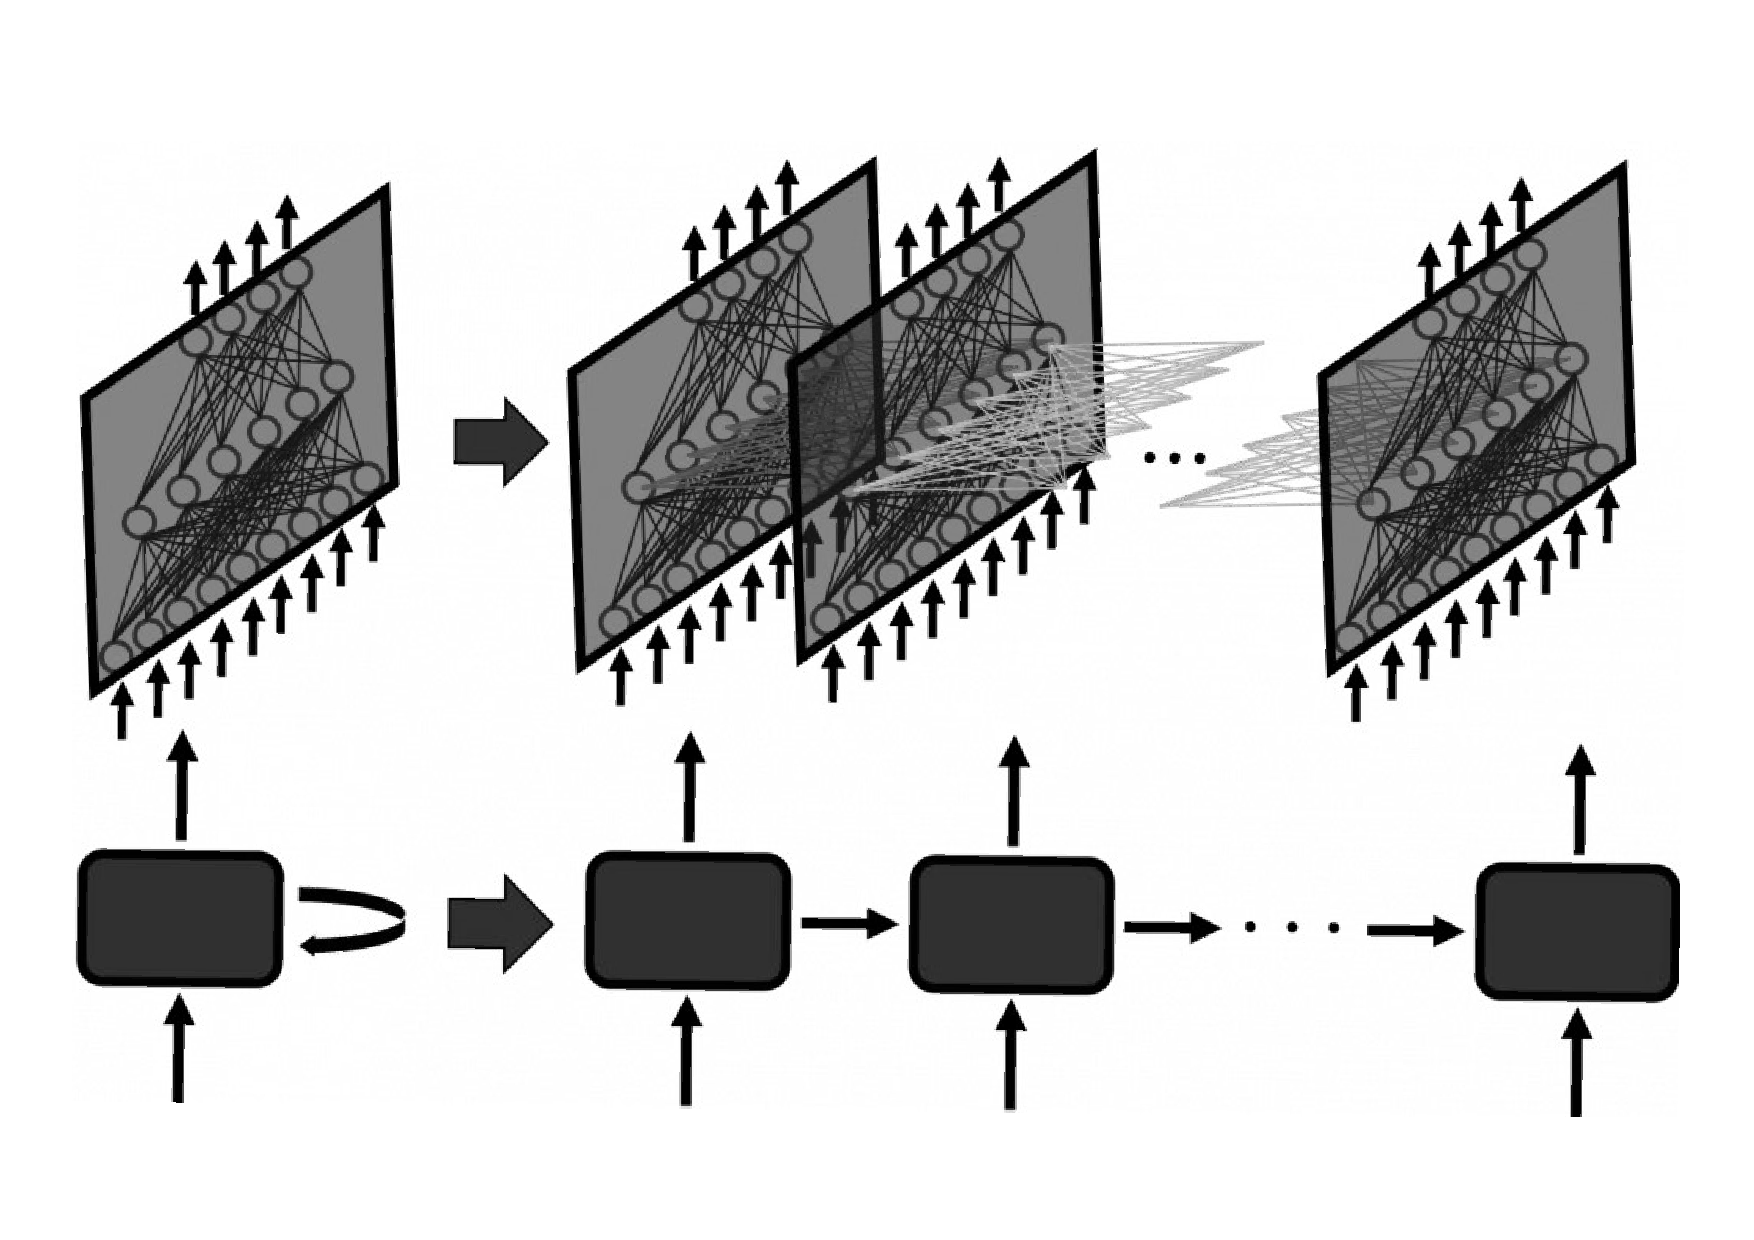
\includegraphics[width=72mm]{Img/chap2_ml/lstm_rnn}
  \bicaption[两层LSTM-RNN的示例]{两层LSTM-RNN的示例。}{The example of two-layer LSTM-RNN.}
  \label{fig:ml_lstm_rnn}
\end{figure}

传统的RNN很容易出现梯度消失现象,这是因为梯度连乘导致长时间神经元的参数更新非常缓慢。LSTM-RNN是一种特殊的RNN,由\citet{hochreiter1997long}提出。LSTM-RNN通过引入历史时间步的神经元状态并更新当前时间步神经元隐藏层的输出,将不需要的信息去掉,解决了梯度消失和梯度爆炸问题。RNN只更新历史一个时间步的状态,而LSTM-RNN可以学习到什么时候以及多长时间遗忘和保存某些信息。LSTM-RNN被广泛应用于文本生成、语音识别、机器翻译、图像描述和视频标记等。图\ref{fig:ml_lstm_rnn}绘制了两层的LSTM-RNN。

为了展示LSTM–RNN如何工作,将图\ref{fig:ml_lstm_rnn}中的LSTM神经元展开,从而得到LSTM神经元结构图(见图\ref{fig:ml_lstm_cell})。图\ref{fig:ml_lstm_cell}中,$\Vector{x}_t$为在时间步为$t$时的输入信号,$\Vector{h}_{t}$为时间步为$t$时的隐藏层状态,$\Vector{h}_{t-1}$为时间步为$t-1$时的隐藏层状态。$\Vector{g}_t=\tanh(\Vector{U}_g\Vector{x}_t+\Vector{V}_g\Vector{h}_{t-1}+\Vector{b}_g)$。$\tanh$为双曲正切函数,$\Vector{i}_t$为输入门,$\Vector{f}_t$为遗忘门,$\Vector{o}_t$为输出门。 $\Vector{c}_t$表示时间步为$t$时单元状态,$\Vector{c}_{t-1}$ 表示时间步为$t-1$时单元状态。$\bigodot$表示元素相乘。黑色方块代表循环阶段。这些神经元具有各种组件,分别为具有记忆单元的输入门、自循环连接的神经元、遗忘门和输出门。记忆单元类似于一个累加器,可以学习序列中的长期依赖关系,从而使优化变得更加容易。同时,每个单元格由三个乘法单元控制,即输入门、输出门和遗忘门,这些决定了是忘记过去单元状态还是将输出传递到之后的状态,从而使LSTM神经元能够长期存储和访问信息。

\begin{figure}[!htbp]
  \centering
  \noindent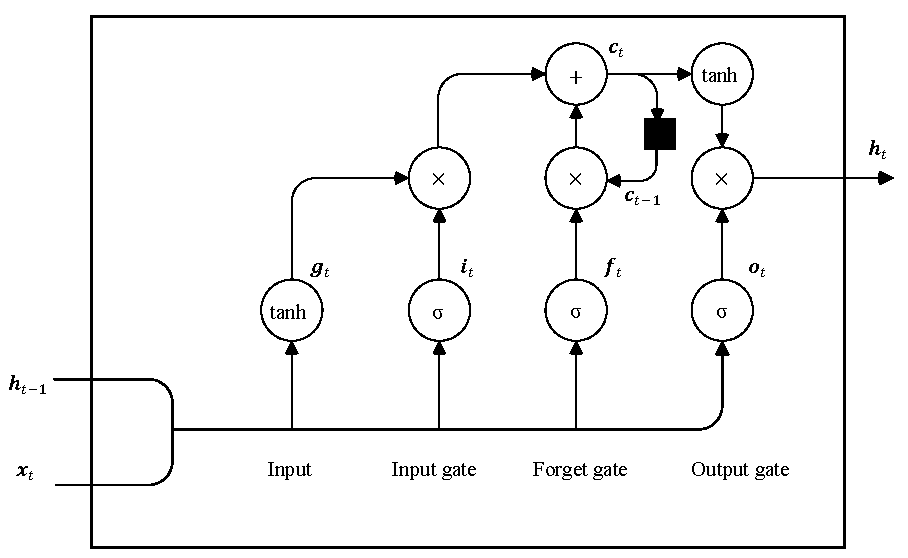
\includegraphics[width=0.75\textwidth]{Img/chap2_ml/lstm_cell}
  \bicaption[LSTM神经元示意图]{LSTM神经元示意图。}{An LSTM cell diagram.}
  \label{fig:ml_lstm_cell}
\end{figure}

LSTM神经元具体工作机制如下:
\begin{enumerate}
  \item[(a)] 首先将序列值$\Vector{x}_t$与神经元$\Vector{h}_{t-1}$作为先前输出,该组合输入的第一步会通过$\tanh(\cdot)$层进行压缩,即$\Vector{g}_t=\tanh(\Vector{U}_g \Vector{x}_t+\Vector{V}_g\Vector{h}_{t-1}+\Vector{b}_g)$,其中$\Vector{U}_g$和$\Vector{V}_g$分别代表输入和前一个神经元的输出的权重,$\Vector{b}_g$表示输入的偏置。$\Vector{g}_t\subset(-1,1)$。第二步此组合输入通过输入门。输入门是一层$\sigma(\cdot)$激活节点,其输出乘以压缩的输入。这些输入门$\sigma(\cdot)$可“杀死”输入向量中不需要的任何元素。$\sigma(\cdot)$函数的输出值$\Vector{i}_t=\sigma(\Vector{U}_i \Vector{x}_t+\Vector{V}_i\Vector{h}_{t-1}+\Vector{b}_i)$,$\Vector{i}_t\subset(0,1)$。其中$\Vector{U}_i$、$\Vector{V}_i$ 和$\Vector{b}_i$均是需要学习的参数,$\Vector{i}_t\subset(0,1)$。将输入连接到这些节点的权重以输出接近于零的值,从而“关闭”某些输入值;或者相反,输出接近于1以“记住”其他值。LSTM神经元输入部分的输出可以由$\Vector{g}_t\bigodot\Vector{i}_t$得到,其中$\bigodot$表示元素相乘。
  \item[(b)] 通过这个单元的数据流的下一步是遗忘循环门,可表示为$\Vector{f}_t=\sigma(\Vector{U}_f\Vector{x}_t+\Vector{V}_f\Vector{h}_{t-1}+\Vector{b}_f)$。其中$\Vector{f}_t\subset(0,1)$,$\Vector{U}_f$、$\Vector{V}_f$和$\Vector{b}_f$分别为两个可调节的权重参数和一个权重值。LSTM神经元有一个内部状态变量$\Vector{c}_t$。这个变量滞后一个时间步,即$\Vector{c}_{t-1}$被添加到输入数据中以创建一个有效的循环层,即$\Vector{c}_{t-1}\bigodot\Vector{f}_t$。$\Vector{c}_t$可表达为$\Vector{c}_{t-1}\bigodot\Vector{f}_t+\Vector{g}_t\bigodot\Vector{i}_t$,这种加法运算而不是乘法运算有助于降低梯度消失的风险。然而,这个循环是由遗忘门控制的,它的工作原理与输入门相同,有助于网络学习哪些状态变量应该被“记住”或“忘记”。
  \item[(c)] 最后,获得一个输出层,由$\tanh(\cdot)$压缩函数控制。这个门决定了哪些值被允许作为神经元$h_t$的输出$\Vector{o}_t$。$\Vector{o}_t=\sigma(\Vector{U}_o\Vector{x}_t+\Vector{V}_o\Vector{h}_{t-1}+\Vector{b}_o)$,$\Vector{o}_t\subset(0,1)$。$\Vector{U}_o$、$\Vector{V}_o$和$\Vector{b}_o$为输出门中一系列可学习的参数。新的隐藏层$\Vector{h}_t$可通过$\tanh(\Vector{c}_t)\Vector{o}_t$计算得到。最后一层的输出$\Vector{h}_n$会连接到一个传统的全连接神经网络,表达为$\Vector{y}=\Vector{W}_d\Vector{h}_n+\Vector{b}_d$。其中$\Vector{y}$作为神经网络的输出,$\Vector{W}_d$和$\Vector{b}_d$分别为权重和偏置。
\end{enumerate}

总体来看,整个LSTM-RNN的运行过程可描述如下。首先,将一系列的时间序列数据$\Vector{X}=\{\Vector{x}_1,\Vector{x}_2,\cdots,\Vector{x}_n\}$作为输入,其中$\Vector{x}_t$是时间步$t$的输入数据。在堆叠的LSTM层中,下一层接收上一层的输出$\Vector{h}=\{\Vector{h}_1,\Vector{h}_2,\cdots,\Vector{h}_n\}$,$\Vector{h}$作为下一层的输入。最后一层使用全连接层,可表达为$\Vector{y}=\Vector{W}_d\Vector{h}_n+\Vector{b}_d$。

\section{训练前的必要准备}\label{sec:ml_prepare}

开展机器学习,首先需要将收集的资料进行整理分析,得到满足目标任务的特征因子。利用滑动窗口法将这些特征因子转化为监督学习数据集。然后,对监督学习数据集进行划分和归一化处理。有时,数据集划分和归一化处理不分前后次序。在优化算法时,需要选择合适的性能度量指标、优化目标函数、优化器等。对算法输出结果进行分析时,还会涉及到算法是否出现过拟合或欠拟合的问题。

\subsection{滑动窗口法}\label{sec:ml_slide}

本论文中选择的数据集(太阳黑子、泉流量、地震数值预测)都是时间序列数据。历史时间序列数据$\{\Vector{x}_{t-M+1},\Vector{x}_{t-M+2},\ldots,\Vector{x}_{t}\}$作为预测下$N$个时间步$\{\Vector{x}_{t+1},\Vector{x}_{t+2},\ldots,\Vector{x}_{t+N}\}$的输入。需要将原始数据集转化为监督学习数据集。监督学习数据集的生成可采用滑动窗口法。图\ref{fig:slide_window}绘制了滑动窗口法的过程。其中,将时间序列中输入时间窗口$M$个观测值作为输入,输出时间窗口$N$个观测值作为输出。将窗口一次滑动一个时间步,对整个原始数据集重复此过程,最终可获得监督学习数据集。

\begin{figure}[!htbp]
  \centering
  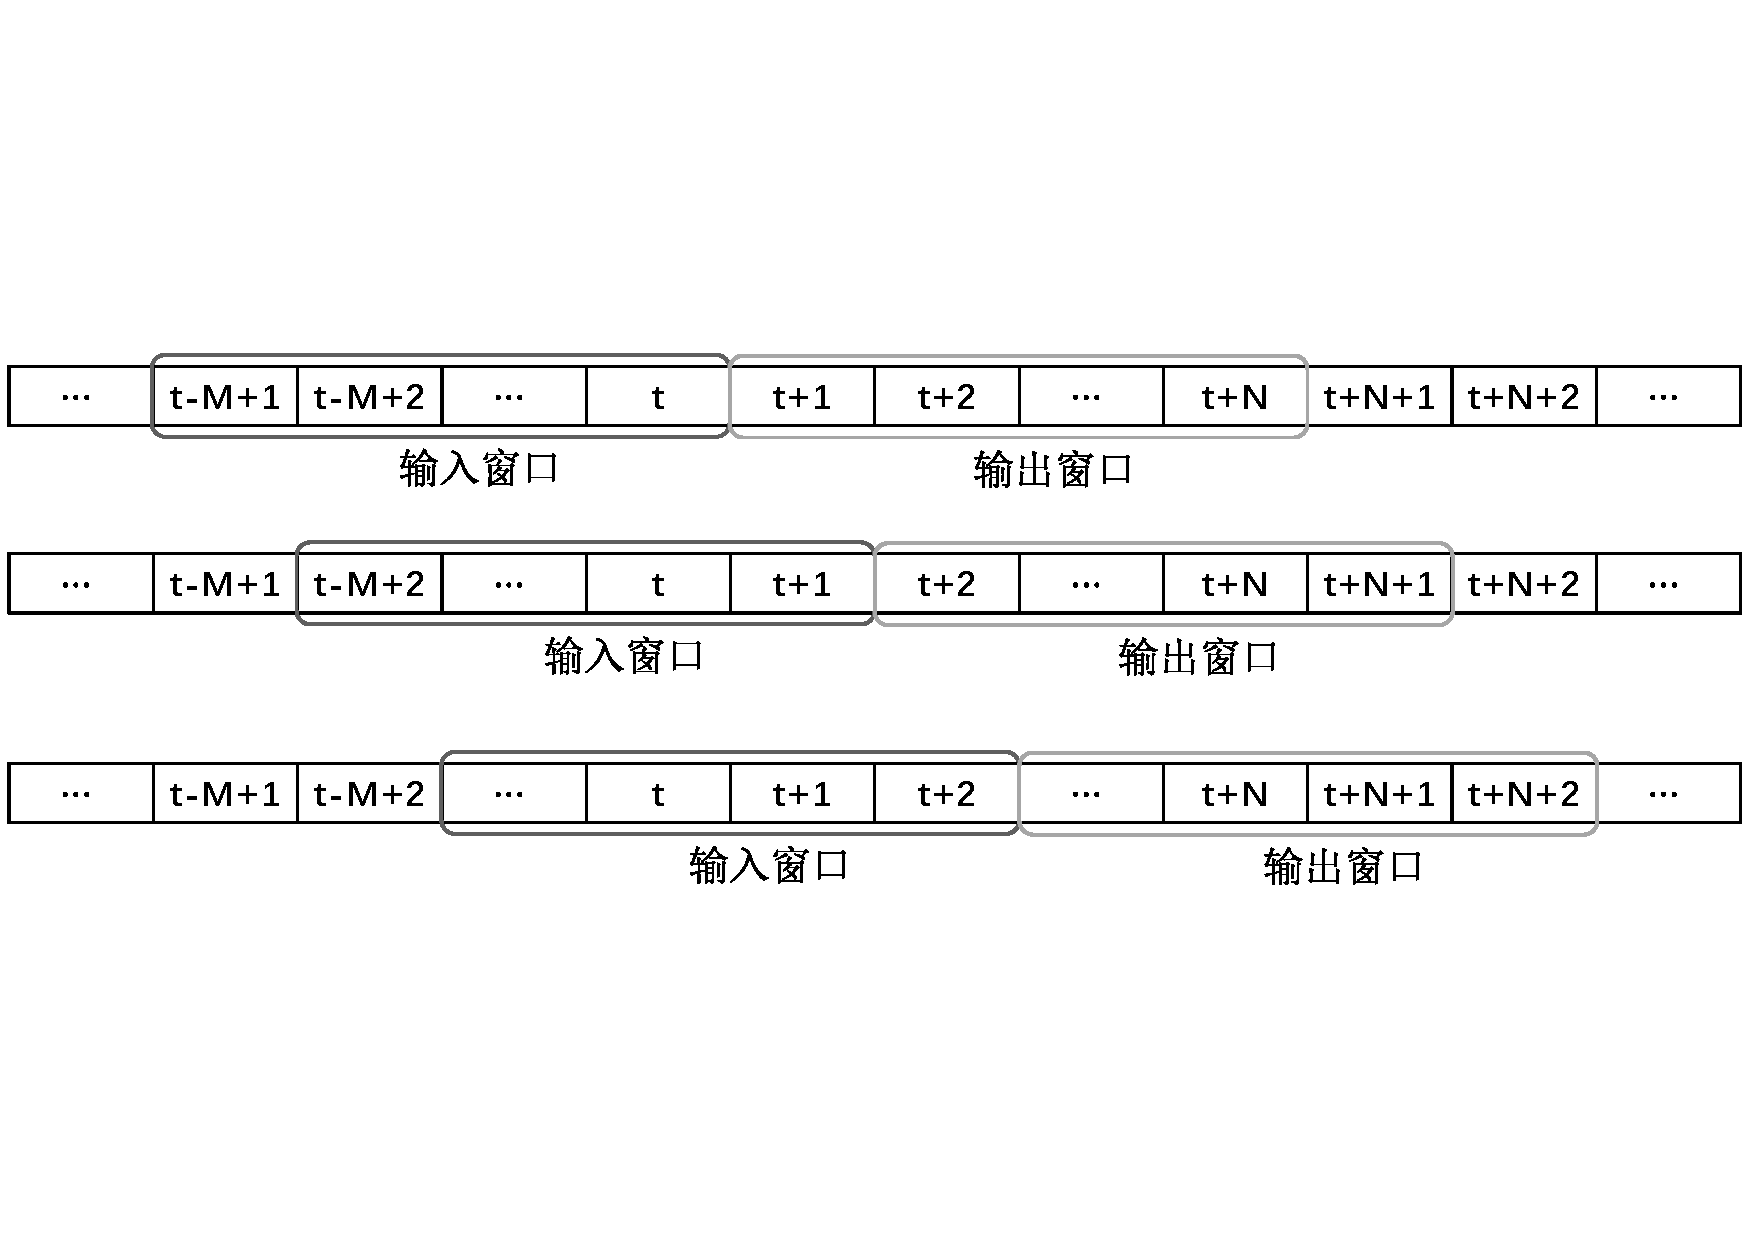
\includegraphics[width=\textwidth]{Img/chap2_ml/slide_window.pdf}
  \bicaption[滑动窗口法]{滑动窗口法的过程。每一行是时间序列数据集。方框中每个数字代表一个时间步。输入窗口和输出窗口在整个可用的数据集中按月/年滑动。}{The process of the sliding window method. Each row is time series dataset. Each number in the box represents a time step. The input and output windows monthly/yearly slide basis on entire available dataset.}
  \label{fig:slide_window}
\end{figure}

\subsection{数据归一化}\label{sec:ml_scaler}

将数据喂给神经网络之前,需要对其进行归一化(Normalization)处理。目的是使预处理的数据被限定在一定范围内,提高算法精度,并加速算法的收敛速度。目前有2种最常用的归一化方法,分别为:
\begin{enumerate}
  \item[$\circ$] \textbf{线性函数归一化}(Min-Max Scaling)。该方法是一种线性转换的方法, 归一化后的数据值被映射到$[0,1]$之间。转化公式如式下:
  \begin{equation}\adddotsbeforeeqnnum 
    \label{eq:ml_scale_min_max}
    \Vector{X}_{\text{norm}}=\frac{\Vector{X}-\Vector{X}_{\text{min}}}{\Vector{X}_{\text{max}}-\Vector{X}_{\text{min}}}.
  \end{equation}
  其中,$\Vector{X}_{\text{norm}}$是归一化后的数据,$\Vector{X}$是原始观测数据,$\Vector{X}_{\text{min}}$是观测数据中的最小值,$\Vector{X}_{\text{max}}$是观测数据中的最大值。
  \item[$\circ$] \textbf{0均值归一化}(Z-Score Standardization)。0均值归一化方法将原始观测数据集归一化为均值为0、方差1的数据集,归一化公式如下:
  \begin{equation}\adddotsbeforeeqnnum 
    \label{eq:ml_scale_z_score}
    \Vector{X}_{\text{norm}}=\frac{\Vector{X}-\mu}{\sigma}.
  \end{equation}
  其中,$\mu$、$\sigma$分别为原始数据集的均值和方差。该种归一化方式要求原始数据的分布可以被近似为高斯分布。
\end{enumerate}

因本论文所涉及的几种数据集都不满足高斯分布特征,因此统一采用线性函数归一化法。

\subsection{优化器}\label{sec:ml_optimizer}

在寻找最优参数(权重和偏置)的过程中,要使目标函数尽可能地小。这个过程需要计算参数的导数(即梯度),以梯度为指引方向逐步更新参数的值。常见的优化算法如下:
\begin{itemize}
  \item[$\circ$] \textbf{随机梯度下降法}(Stochastic Gradient Descent,简称SGD)。SGD计算过程中基于单个样本,即每读一个数据,则立刻计算代价函数的梯度。
  \item[$\circ$] \textbf{批量梯度下降}(Batch Gradient Descent,简称BGD)。BGD在计算过程中基于整个数据集,即读取所有数据后才会计算代价函数的梯度。
  \item[$\circ$] \textbf{小批量梯度下降}(Mini-Batch Gradient Descent,简称Mini-BGD)。Mini-BGD选择小批量数据更新梯度。SGD、BGD和Mini-BGD三类方法都存在一个问题,即更新方向完全依赖于梯度,容易陷入局部最优。
  \item[$\circ$] \textbf{动量}(Momentum)。Momentum引入了动量的物理概念,使得未来梯度方向与历史关联起来,从而跳出了局部最优。
  \item[$\circ$] \textbf{自适应梯度}(Adaptive Gradient,简称Adagrad)。Adagrad会累加历史所有梯度的平方。
  \item[$\circ$] \textbf{均方根反向传播}(Root Mean Square Propagation,简称RMSprop)。MSProp计算所有梯度的平均值。Adagrad和RMSprop都属于自适应学习率方法,训练过程中的步长(即学习率)时刻在调整。
  \item[$\circ$] \textbf{Adam}(Adaptive Moment Estimation)。Adam融合了RMSProp和Adagrad,通过组合两者的优点,实现参数空间的高效搜索。
\end{itemize}

本论文在训练神经网络时使用了Adam优化算法,它由\citet{kingma2014adam}提出。Adam简单高效,不需要消耗过多内存,尤其适用于具有大量的数据和很多参数的问题中。Adam第一分量(\ref{eq:m_t})和第二分量(\ref{eq:v_t})分别表示为:
\begin{equation}\adddotsbeforeeqnnum 
  \label{eq:m_t}
  m_t = \beta_1 m_{t-1}+(1-\beta_1)g_t.
\end{equation}
\begin{equation}\adddotsbeforeeqnnum 
  \label{eq:v_t}
  v_t = \beta_2 m_{t-1}+(1-\beta_2)g^2_t.
\end{equation}
其中,$m_t$和$v_t$分别是第一分量和第二分量的估计值。$m_t$和$v_t$均被初始化为0。当衰减值很小时,梯度会出现偏差。利用式\ref{eq:m_t1}和式\ref{eq:v_t1},通过修正偏置来解决偏差问题。
\begin{equation}\adddotsbeforeeqnnum 
  \label{eq:m_t1}
  \hat{m}_t = \frac{m_t}{1-\beta_1^t}.
\end{equation}
\begin{equation}\adddotsbeforeeqnnum 
  \label{eq:v_t1}
  \hat{v}_t = \frac{v_t}{1-\beta_2^t}.
\end{equation}
其中,$\beta_1$默认值为$0.9$, $\beta_2$默认值为$0.999$。在修正了偏置后,权重也得以修正(见式\ref{eq:theta})。
\begin{equation}\adddotsbeforeeqnnum 
  \label{eq:theta}
  \theta_{t+1}=\theta_t-\frac{\eta}{\sqrt{\hat{v}_t}+\epsilon}m_t.
\end{equation}
其中,$\epsilon$默认值为$10^{-8}$。

\subsection{优化目标函数}\label{sec:ml_loss}

在学习过程中,算法会通过某个指标寻找最优权重参数,这个指标为代价函数(Cost Function)。代价函数能够很直观地呈现数据集的拟合程度。训练算法的过程,也就是最小化预测值与目标值差距的过程,或者说最小化代价函数的过程。这里需要仔细区分损失函数(Loss Function)、代价函数和目标函数:
\begin{itemize}
  \item[(a)] \textbf{损失函数}。损失函数针对单个样本,计算的是单个样本的误差,损失函数可表述为$L(\Vector{y}_i-f(\Vector{x}_i))$。通常损失函数有以下几种:
  \begin{enumerate}
    \item[$\circ$] 绝对损失函数:
    \begin{equation}\adddotsbeforeeqnnum
      \label{eq:ml_loss_absolute}
      L(\Vector{y}_i,f(\Vector{x}_i))=|\Vector{y}_i-f(\Vector{x}_i)|.
    \end{equation}
    \item[$\circ$] 平方损失函数:
    \begin{equation}\adddotsbeforeeqnnum
      \label{eq:ml_loss_mean}
      L(\Vector{y}_i,f(\Vector{x}_i))=(\Vector{y}_i-f(\Vector{x}_i))^2.
    \end{equation}
    \item[$\circ$] 0-1损失函数:
    \begin{equation}\adddotsbeforeeqnnum
      \label{eq:ml_loss_01}
      L(\Vector{y}_i,f(\Vector{x}_i))=
      \begin{cases}
        0, \Vector{y}_i=f(\Vector{x}_i)\\
        1, \Vector{y}_i\neq f(\Vector{x}_i)
      \end{cases}.
    \end{equation}
    \item[$\circ$] 交叉熵损失函数:
    \begin{equation}\adddotsbeforeeqnnum
      \label{eq:ml_loss_cross_entropy}
      L(\Vector{y}_i,f(\Vector{x}_i))=-\Vector{y}_i\log f(\Vector{x}_i).
    \end{equation}
  \end{enumerate}
  通常,式\ref{eq:ml_loss_absolute}和式\ref{eq:ml_loss_mean}被用在回归问题上,式\ref{eq:ml_loss_absolute}被用在二分类问题上,式\ref{eq:ml_loss_cross_entropy}被用在多分类问题上。

  \item[(b)] \textbf{代价函数}。与损失函数不同的是,代价函数针对的是整个训练样本,是所有样本误差的平均值,也就是损失函数的平均值,一般被称作经验风险最小化函数,表达式为
  \begin{equation}\adddotsbeforeeqnnum
    \label{eq:ml_loss_experience}
    J=\frac{1}{N}\sum_{i=1}^{N}L(\Vector{y}_i,f(\Vector{x}_i)).
  \end{equation}
  但经验风险过小在多数情况下会出现过拟合,而过拟合的原因是$f(\Vector{X})$太过复杂。

  \item[(c)] \textbf{目标函数}。对于小样本,用经验风险估计期望经常不太理想,需要对其进行矫正。结构风险最小化是为了抗过拟合而提出的策略。结构风险在经验风险上加入了表示算法复杂度的正则化项$\lambda J(f)$,因此结构方程为
  \begin{equation}\adddotsbeforeeqnnum
    \label{eq:ml_loss_structure}
    J_{\lambda}=\frac{1}{N}\sum_{i=1}^{N}L(\Vector{y}_i,f(\Vector{x}_i))+\lambda J(f).
  \end{equation}
  最终的优化函数为$\min J_{\lambda}$,此函数又被称作目标函数。
\end{itemize}

\subsection{性能度量}\label{sec:ml_performance}

机器学习中,通常将数据集划分为训练集和测试集,还假设这两种数据集同分布。一般在训练集上构建算法,寻找最优算法,然后使用测试集验证算法的实际预测能力。如果一个算法能够对未见样本(即测试集)做出准确预测,则认为该算法能够从训练集泛化到测试集。泛化能力指预测测试集的能力,获得较强的泛化能力是机器学习的最终目标。

如果算法只能正确识别已有的训练集,而预测测试集时出现很大的偏差,那有可能只学习到了训练集中的无关紧要的细节(如噪声)。需要注意的是,仅仅用训练集去学习和评价参数,常常会导致算法只可以用来处理某种数据集,对于其他数据集难以正确处理。

对算法的泛化性能进行评估,需要衡量算法泛化能力的评价标准,即性能度量(Performance Measure)。通常,使用不同的性能度量指标,评判结果会有差异。学习的最终目标是,预测结果与真实值尽可能地接近。性能度量指标有:
\begin{enumerate}
  \item[$\circ$] 均方误差(Mean Squared Error,简称MSE)。数学公式为:
  \begin{equation}\adddotsbeforeeqnnum
    \label{eq:ml_mse}
    \text{MSE}=\frac{1}{m}\sum_{i=1}^{m}(f(\Vector{x}_i)-\Vector{y}_i)^2.
  \end{equation}
  \item[$\circ$] 绝对误差(Mean Absolute Error,简称MAE)。数学公式为:
  \begin{equation}\adddotsbeforeeqnnum
    \label{eq:ml_mae}
    \text{MAE}=\frac{1}{m}\sum_{i=1}^{m}|f(\Vector{x}_i)-\Vector{y}_i|.
  \end{equation}
  \item[$\circ$] 均方根误差(Root Mean Absolute Error,简称RMSE)。数学公式为:
  \begin{equation}\adddotsbeforeeqnnum
    \label{eq:ml_rmse}
    \text{RMSE}=\sqrt{\frac{1}{m}\sum_{i=1}^{m}(f(\Vector{x}_i)-\Vector{y}_i)^2}.
  \end{equation}
  \item[$\circ$] 平均绝对百分比误差(Mean Absolute Percentage Error,简称MAPE)。数学公式为
  \begin{equation}\adddotsbeforeeqnnum
    \label{eq:ml_mape}
    \text{MAPE}=\frac{100\%}{m}\sum_{i=1}^{m}|\frac{f(\Vector{x})_i-\Vector{y}_i}{\Vector{y}_i}|.
  \end{equation}
  \item[$\circ$] 交叉熵误差(Cross Entropy Error,简称CEE)。数学公式为:
  \begin{equation}\adddotsbeforeeqnnum
    \label{eq:ml_cee}
    \text{CEE}=-\sum_{i=1}^{m}(\Vector{y}_i\log f(\Vector{x}_i)).
  \end{equation}
  \item[$\circ$] 准确度(Accuracy)。数学公式为:
  \begin{equation}\adddotsbeforeeqnnum
    \label{eq:ml_acc}
    \text{Accuracy}=\frac{1}{m}\sum_{i=1}^{m}(\Vector{y}_i == f(\Vector{x}_i)).
  \end{equation}
\end{enumerate}
在处理回归问题时,本论文采用MSE作为损失函数,RMSE作为预测的误差。

\subsection{欠拟合和过拟合}\label{sec:ml_fitting}

这里对欠拟合和过拟合做出解释。欠拟合(Under-Fitting)也称欠学习,直观表现是算法训练得到的算法在训练集上表现差,未学到数据的规律。引起欠拟合的原因可能有:
\begin{enumerate}
  \item[$\circ$] 算法本身过于简单。例如,数据本身是非线性的,但使用了线性算法;
  \item[$\circ$] 特征数太少,无法正确的建立统计关系。
\end{enumerate}

过拟合(Over-Fitting)也称过学习,它的直观表现是算法在训练集上表现良好,但在测试集上表现不好,泛化性能差。过拟合是在算法参数拟合过程中由于训练数据包含抽样误差,在训练时复杂的算法将抽样误差也进行了拟合。所谓抽样误差,是指抽样得到的样本集和整体数据集之间的偏差。直观来看,引起过拟合可能的原因有:
\begin{enumerate}
  \item[$\circ$] 算法本身过于复杂,以至于拟合了训练样本集中的噪声。需要选用更简单的算法,或者对算法进行简化;
  \item[$\circ$] 训练样本太少或缺乏代表性。需要增加样本数或增加样本的多样性;
  \item[$\circ$] 算法拟合了噪声。需要剔除噪声或者改用对噪声不敏感的算法。
\end{enumerate}

过拟合是有监督机器学习算法长期以来需要面临的一个问题。表\ref{tab:ml_overfit}给出了实际应用时判断过拟合与欠拟合的准则。
\begin{table}[!htbp]
  \bicaption[过拟合与欠拟合的判断标准]{过拟合与欠拟合的判断标准。}{The criterion for under-fitting and over-fitting.}
  \label{tab:ml_overfit}
  \centering
  \footnotesize
  \begin{tabular}{ccc}
    \toprule
    训练集上的表现 & 测试集上的表现 & 判断 \\
    \midrule
    欠佳 & 欠佳 & 欠拟合 \\
    良好 & 欠佳 & 过拟合 \\
    良好 & 良好 & 适度拟合 \\
    \bottomrule
  \end{tabular}
\end{table}

还可以从偏差和方差的角度来看待欠拟合和过拟合。算法的泛化误差来源于三部分,即偏差(Bias)、方差(Variance)和噪声(Noise)。偏差度量了学习算法的期望预测值与真实值的偏离程度,即刻画了学习算法本身的拟合能力。假设输入特征向量为$\Vector{X}$,输出为$Y$,实际输出为$Y^{\prime}$,要拟合的目标函数为$f(\Vector{X})$,训练的函数为$\hat{f}(\Vector{X})$,则偏差为:
\begin{equation}\adddotsbeforeeqnnum
  \label{eq:ml_bias}
  \text{Bais}^2(\Vector{X})=(\hat{f}(\Vector{X})-Y)^2.
\end{equation}
高偏差意味着算法本身的输出值与期望值差距大,导致欠拟合。

与偏差不同,方差度量了训练集的变动影响算法性能的程度,即刻画了数据扰动所造成的影响。它是对训练样本的小波动敏感而导致的误差。方差可以理解为算法的波动程度。根据概率论中方差的定义:
\begin{equation}\adddotsbeforeeqnnum
  \label{eq:ml_variance}
  \text{Variance}(\Vector{X})=E[(\hat{f}(\Vector{X})-f(\Vector{X}))^2].
\end{equation}
高方差意味着算法本身与期望的算法差距大,从而导致过拟合。

除了偏差与方差,噪声也会影响到算法性能的好坏。噪声表达了在当前任务上任何学习算法所能达到的期望泛化误差的下界,即刻画了学习问题本身的难度。期望预测值与真实值之间的误差称为噪声,即
\begin{equation}\adddotsbeforeeqnnum
  \label{eq:ml_noise}
  \text{Noise}(\Vector{X})=E[(Y^{\prime}-Y)^2].
\end{equation}
当存在噪声时,复杂的算法会尽量覆盖噪声,即产生了过拟合。这样,即使训练误差很小,由于没有描绘真实的数据趋势,测试误差反而更大。还有一种情况,如果数据是由未知的非常复杂的系统产生的,实际上有限的数据很难去“代表”这个复杂系统。采用不恰当的数据集拟合,算法性能会很差,因为部分数据在不恰当的复杂假设下就像是“噪声”,从而产生过拟合。

综上,泛化误差可分解为偏差、方差和噪声,即
\begin{equation}\adddotsbeforeeqnnum
  \label{eq:ml_error}
  \text{Error}(\Vector{X})=\text{Bais}^2(\Vector{X})+\text{Variance}(\Vector{X})+\text{Noise}(\Vector{X}).
\end{equation}
以上分解说明,泛化性能是由学习算法的能力、数据的充分性以及学习任务本身的难度共同决定。一般来讲,噪声难以避免,更难以被剔除。为了获得更好的泛化性能,需要同时减小偏差(能充分拟合数据)和方差(数据扰动产生的影响小)。

\begin{figure}[!htbp]
  \centering
  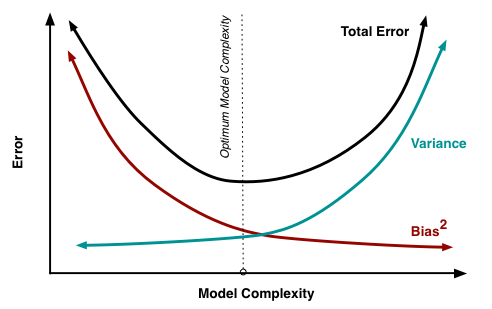
\includegraphics[width=0.6\textwidth]{Img/chap2_ml/bias.png}
  \bicaption[AIC信息准则]{AIC信息准则。}{Akaike information criterion.}
  \label{fig:ml_bias}
\end{figure}

但是偏差和方差是有冲突的。图\ref{fig:ml_bias}给出了AIC信息准则(Akaike Information Criterion),又称赤池信息准则,表达了泛化误差与偏差、方差的关系。它建立在熵的概念基础上,可以权衡所估计算法的复杂度和此算法拟合数据的优良性。当算法训练不足时,训练数据的特征没有被很好地拟合,会产生较大偏差和较小方差。当算法得到进一步训练时,偏差会逐渐减小,而方差会逐渐增大。当算法被充分训练之后,学习器的拟合能力非常强,会出现较小的偏差和较大的方差,算法会将训练数据中的所有特征(包括噪声)都学习到,此时就会发生过拟合。

学习率和批量处理大小(Batch-Size)都是影响算法优化效率和泛化能力的超参数。在实际训练过程中,会观察算法每一次更新过程中测试集误差的变化趋势。当测试集误差在指定的循环次数范围内未能有进一步改善的空间,算法会被人为终止,这种策略也被称作“早停”(Early Stopping)。这种方法简单有效,是深度学习中最常见的正则化策略之一。

\subsection{计算工具与平台}\label{sec:ml_computer}

论文中涉及的数据分析全部基于Python中的开源库编码实现。开源库主要包括Tensorflow2.0、Scikit-learn、Numpy、Pandas、Matplotlib、Julian等,其中Tensorflow2.0用来构建神经网络算法,Scikit-learn用来构建常用的机器学习算法,Numpy和Pandas主要针对数据进行预处理,Matplotlib则是在可视化结果时使用,Julian将数据中的序列数据转化为日期。论文计算任务在本地服务器(1$\times$GPU1080Ti)上完成。

\section{小结}\label{sec:ml_conclusion}

本章详细介绍了机器学习的理论基础以及相关优化的概念和方法。第\ref{sec:ml}节介绍了不同的机器学习算法的基础理论,包括LR、KNN、DT、RF、SVR、GBRT、ETR、CNN、LSTM-RNN。第\ref{sec:ml_prepare}节说明了算法需要的前期准备,包括基于滑动窗口法获取监督学习数据集、数据划分、归一化、优化器和优化函数的选择、性能度量标准、欠拟合和过拟合等。

